\documentclass[12pt,a4paper]{article}
%\usepackage{fontspec, xunicode, xltxtra}  
%\setmainfont{Hiragino Sans GB}  
%\usepackage{xeCJK}
%\setCJKmainfont[BoldFont=STZhongsong, ItalicFont=STKaiti]{STSong}
%\setCJKsansfont[BoldFont=STHeiti]{STXihei}
%\setCJKmonofont{STFangsong}

%使用Xelatex编译

% 设置页面
%==================================================
\linespread{2} %行距
% \usepackage[top=1in,bottom=1in,left=1.25in,right=1.25in]{geometry}
% \headsep=2cm
% \textwidth=16cm \textheight=24.2cm
%==================================================

% 其它需要使用的宏包
%==================================================
\usepackage[colorlinks,linkcolor=blue,anchorcolor=red,citecolor=green,urlcolor=blue]{hyperref} 
\usepackage{tabularx}
\usepackage{authblk}         % 作者信息
\usepackage{algorithm}     % 算法排版
\usepackage{amsmath}     % 数学符号与公式
\usepackage{amsfonts}     % 数学符号与字体
\usepackage{mathrsfs}      % 花体
\usepackage[framemethod=TikZ]{mdframed}

\usepackage{graphicx} 
\usepackage{graphics}
\usepackage{color}
\usepackage{xcolor}

\usepackage{fancyhdr}       % 设置页眉页脚
\usepackage{fancyvrb}       % 抄录环境
\usepackage{float}              % 管理浮动体
\usepackage{geometry}     % 定制页面格式
\usepackage{hyperref}       % 为PDF文档创建超链接
\usepackage{lineno}          % 生成行号
\usepackage{listings}        % 插入程序源代码
\usepackage{multicol}       % 多栏排版
%\usepackage{natbib}         % 管理文献引用
\usepackage{rotating}       % 旋转文字,图形,表格
\usepackage{subfigure}    % 排版子图形
\usepackage{titlesec}       % 改变章节标题格式
\usepackage{moresize}   % 更多字体大小
\usepackage{anysize}
\usepackage{indentfirst}  % 首段缩进
\usepackage{booktabs}   % 使用\multicolumn
\usepackage{multirow}    % 使用\multirow

\usepackage{wrapfig}
\usepackage{titlesec}     % 改变标题样式
\usepackage{enumitem}
\usepackage{aas_macros}
\usepackage{harpoon}   %矢量符号
\usepackage{tcolorbox}

\newcommand{\myvec}[1]%
   {\stackrel{\raisebox{-2pt}[0pt][0pt]{\small$\rightharpoonup$}}{#1}}  %矢量符号
\renewcommand{\vec}[1]{\boldsymbol{#1}}
\newcommand{\me}{\mathrm{e}}
\newcommand{\mi}{\mathrm{i}}
\newcommand{\dif}{\mathrm{d}}
\newcommand{\tabincell}[2]{\begin{tabular}{@{}#1@{}}#2\end{tabular}}

\def\kpc{{\rm kpc}}
\def\km{{\rm km}}
\def\cm{{\rm cm}}
\def\TeV{{\rm TeV}}
\def\GeV{{\rm GeV}}
\def\MeV{{\rm MeV}}
\def\GV{{\rm GV}}
\def\MV{{\rm MV}}
\def\yr{{\rm yr}}
\def\s{{\rm s}}
\def\ns{{\rm ns}}
\def\GHz{{\rm GHz}}
\def\muGs{{\rm \mu Gs}}
\def\arcsec{{\rm arcsec}}
\def\K{{\rm K}}
\def\microK{\mu{\rm K}}
\def\sr{{\rm sr}}
\newcolumntype{p}{D{,}{\pm}{-1}}

\renewcommand{\figurename}{Fig.}
\renewcommand{\tablename}{Tab.}

\renewcommand{\arraystretch}{1.5}

\setlength{\parindent}{0pt}  %取消每段开头的空格

\newcounter{theo}[section]\setcounter{theo}{0}
\renewcommand{\thetheo}{\arabic{section}.\arabic{theo}}
\newenvironment{theo}[2][]{%
\refstepcounter{theo}%
\ifstrempty{#1}%
{\mdfsetup{%
frametitle={%
\tikz[baseline=(current bounding box.east),outer sep=0pt]
\node[anchor=east,rectangle,fill=blue!20]
{\strut Theorem~\thetheo};}}
}%
{\mdfsetup{%
frametitle={%
\tikz[baseline=(current bounding box.east),outer sep=0pt]
\node[anchor=east,rectangle,fill=blue!20]
{\strut Theorem~\thetheo:~#1};}}%
}%
\mdfsetup{innertopmargin=10pt,linecolor=blue!20,%
linewidth=2pt,topline=true,%
frametitleaboveskip=\dimexpr-\ht\strutbox\relax
}
\begin{mdframed}[]\relax%
\label{#2}}{\end{mdframed}}



\title{Build-Up of Magnetic Fields}
\author{}
\date{\today}
\begin{document}

\maketitle

\section{The Dynamo Problem}
\cite{2015bps..book.....C} The magnetic field on Earth is about \textcolor{cyan}{one gauss} and most of the planets, with the exception of Venus and possibly Mars, also exhibit magnetic fields of varying strength. The average magnetic field of the Sun is of the order of a few gauss, but locally it can be much stronger, reaching values up to a few thousand gauss in sunspots. Magnetic fields of normal stars also reach values around $1,000$ G, but those of compact stars may be extremely intense by comparison: the field of a magnetized white dwarf is typically of the order of a few million gauss and the magnetic fields of pulsars fall in the range of $10^{12}$ G. The galactic magnetic field, on the contrary, is extremely weak, of the order of a few microgauss.

To a first approximation, the external fields of planets and stars are well approximated by magnetic dipoles, but, as we shall see, the internal fields are likely to have a very different structure.

Cosmic plasmas are not perfect conductors and are therefore subject to ohmic decay, even if their resistivity is very small, as shown by the induction equation describing the time evolution of magnetic fields 
\begin{equation}
\frac{\partial \vec{B}}{\partial t} = \nabla \times (\vec{U} \times \vec{B}) +\eta \nabla^2 \vec{B} ~.
\end{equation}
The two terms on the right are associated with very different timescales given, respectively, by $\tau_f = \mathcal{L/U}$, the fluid or convective scale and $\tau_d = \mathcal L^2/\eta$, the diffusive or dissipative scale. $\mathcal U$ is a typical value of the fluid speed, $\mathcal L$ is the scale of the spatial variation of the magnetic field and $\eta = (c^2/4\pi \sigma)$ is the magnetic diffusivity of the plasma which we will take here to be uniform.

The complete solution of the problem would require the induction equation to be solved at the same time and in parallel with the momentum equation. At the heart of the dynamo problem lies understanding which velocity fields, sustained by the available forces, are capable of supporting a growing, oscillating or steady magnetic field against ohmic decay. It is called \textcolor{red}{kinematic dynamo problem}, where the induction equation is actually decoupled from the equation of motion by assuming a particular form for the velocity field. 

\section{The Anti-Dynamo Theorems}
\cite{2015bps..book.....C} A certain number of two- and three-dimensional theorems can be proven that deny the possibility of producing a magnetic field lasting in time. Common assumptions to all theorems are the incompressibility of the flow, $\nabla \cdot \vec{U} = 0$, and the vanishing of $\vec{U}$, $\vec{B}$ and $\vec{A}$ at infinity.

\begin{theo}[]{}
In cartesian coordinates $[x,y,z]$, it is impossible to generate by dynamo action a z-independent field that vanishes at infinity.
\end{theo}


\begin{theo}[]{}
In cartesian coordinates $[x, y, z]$, a planar flow cannot produce a dynamo effect.
\end{theo}

\begin{theo}[]{}
An axisymmetric magnetic field vanishing at infinity cannot be maintained by dynamo action.
\end{theo}



\section{Phenomenological Theory of Astrophysical Dynamos}
\cite{2015bps..book.....C} 

\subsection{The Generation of Toroidal Fields from Poloidal Ones}

\subsection{The Generation of Poloidal Fields from Toroidal Ones}

\section{Mean-field Electrodynamics}
\cite{2015bps..book.....C} 

\subsection{Simple Solutions of the Dynamo Equations}



\section{The Creation of Magnetic Fields}
\cite{2015bps..book.....C} 

\section{MHD DynamoTheory}
\cite{Plasma2014} The ``solid" planets could not possibly be sufficiently ferromagnetic to account for their magnetism, because the temperatures of their interiors lie above the Curie temperature at which permanent magnetism disappears. The paleomagnetism, the study of magnetic fields ``fossilized" in rocks at the time of their formation in the remote geological past, shows that the Earth's magnetic field has existed at much its present strength for at least the past $3 \times 10^9$ years. In the absence of an internal source of electric currents, magnetic fields contained in a conducting body decay ohmically on a timescale
\begin{equation}
\tau_{\rm ohm} = \mu_0 \sigma L^2 ~,
\end{equation}
where $\sigma$ is the typical electrical conductivity, and $L$ is the typical lengthscale of the body, and this decay timescale is generally very small compared to the inferred lifetimes of astrophysical magnetic fields. 

All astrophysical bodies that contain anomalously long-lived magnetic fields also contain convecting, highly conducting, fluids, and it is the electric currents associated with the motions of these fluids that maintain the observed magnetic fields. The magnetic energy irreversibly lost via ohmic heating is replenished at the rate (per unit volume) $\vec{V} \cdot (\vec{j} \times \vec{B})$: in other words, by the rate of work done against the Lorentz force. The flow field, $\vec{V}$, is assumed to be driven via thermal convention. If the flow is sufficiently vigorous then it is plausible that the energy input to the magnetic field can overcome the losses due to ohmic heating, thus permitting the field to persist over timescales far longer than the characteristic ohmic decay time.

Paleomagnetic data from marine sediment cores shows that the Earth's magnetic field is quite variable, and actually reversed polarity about $700, 000$ years ago. The Earth's magnetic field reverses polarity about once every ohmic decay timescale (i.e., a few times every million years). The Sun's magnetic field exhibits similar behavior, reversing polarity about once every $11$ years. The dynamo magnetic fields (and velocity fields) are essentially chaotic in nature, exhibiting strong random variability superimposed on more regular quasi-periodic oscillations.

The \textcolor{red}{kinematic dynamo theory}, in which the velocity field, $\vec{V}$, is prescribed. It must be assumed that the magnetic field is sufficiently weak that it does not affect the velocity field. The MHD Ohm's law, modified by resistivity is
\begin{equation}
\vec{E} +\vec{V}\times \vec{B} = \eta \vec{j} ~.
\end{equation}
The resistivity $\eta$ is assumed to be a constant. Taking the curl of the previous equation, and making use of Maxwell's equations, 
\begin{equation}
\dfrac{\partial \vec{B}}{\partial t} -\nabla \times (\vec{V}\times \vec{B} ) = \dfrac{\eta}{\mu_0} \nabla^2 \vec{B} ~.
\end{equation}
If the velocity field, $\vec{V}$, is prescribed, and unaffected by the presence of the magnetic field, then the previous equation is essentially a linear eigenvalue equation for the magnetic field, $\vec{B}$.

\section{Homopolar Disk Dynamo}
\cite{Plasma2014} As illustrated in Figure (\ref{fig:homopolar}), it consists of \textcolor{red}{a conducting disk that rotates at some angular frequency $\vec{\Omega}$ about its axis under the action of an applied torque}. A wire, twisted about the axis in the manner shown, makes sliding contact with the disc at $A$, and with the axis at $B$, and carries a current $\vec{I}(t)$. The magnetic field, $\vec{B}$, associated with this current has a flux $\Phi = M I$ across the disc, where $M$ is the mutual inductance between the wire and the rim of the disc. The rotation of the disc in the presence of this flux generates a radial electromotive force
\begin{equation}
\dfrac{\Omega}{2\pi} \Phi = \dfrac{\Omega}{2\pi} MI ~,
\end{equation}
because a radius of the disc cuts the magnetic flux $\Phi$ once every $2\pi/\Omega$ seconds. The equation for $I$ is written
\begin{equation}
L\dfrac{\dif I}{\dif t} +RI = \dfrac{M}{2\pi} \Omega I ~,
\end{equation}
where $R$ is the total resistance of the circuit, and $L$ is its self-inductance. 

Suppose that the angular velocity $\Omega$ is maintained by suitable adjustment of the driving torque. An exponential solution $I(t) = I(0) \exp(\gamma t)$, where
\begin{equation}
\gamma = L^{-1} \left(\dfrac{M}{2\pi} \Omega -R \right) ~.
\end{equation}
We have exponential growth of $I(t)$ - and, hence, of the magnetic field to which it gives rise (i.e., we have dynamo action)- provided that
\begin{equation}
\Omega > \dfrac{2\pi R}{M} 
\label{eq:gamma}
\end{equation}
provided that the disk rotates sufficiently rapidly. Note that the homopolar disk dynamo depends for its success on its built-in axial asymmetry. If the disk rotates in the opposite direction to that shown in Figure \ref{fig:homopolar}, then $\Omega < 0$, and the electromotive force generated by the rotation of the disk always acts to reduce $I$. In this case, dynamo action is impossible (i.e., $\gamma$ is always negative). This is a troubling observation, because most astrophysical objects, such as stars and planets, possess very good axial symmetry. We conclude that if such bodies are to act as dynamos then the asymmetry of their internal motions must somehow compensate for their lack of built-in asymmetry. It is far from obvious how this is going to happen.

Incidentally, although the previous treatment of a homopolar disk dynamo (which is the standard analysis found in most textbooks) is very appealing in its simplicity, it cannot be entirely correct. Consider the limiting situation of a perfectly conducting disk and wire, in which $R = 0$. On the one hand, Equation (\ref{eq:gamma}) yields $\gamma = M \Omega/(2\pi L)$, so that we still have dynamo action. But, on the other hand, the rim of the disk is a closed circuit embedded in a perfectly conducting medium, so the flux freezing constraint requires that the flux, $\Phi$, through this circuit must remain a constant. There is an obvious contradiction. The problem is that we have neglected the currents that flow azimuthally in the disc: that is, the currents that control the diffusion of magnetic flux across the rim of the disk. These currents become particularly important in the limit $R \rightarrow \infty$.

The previous paradox can be resolved by supposing that the azimuthal current,















%===========================================================================================================================
\begin{figure*}
\centering
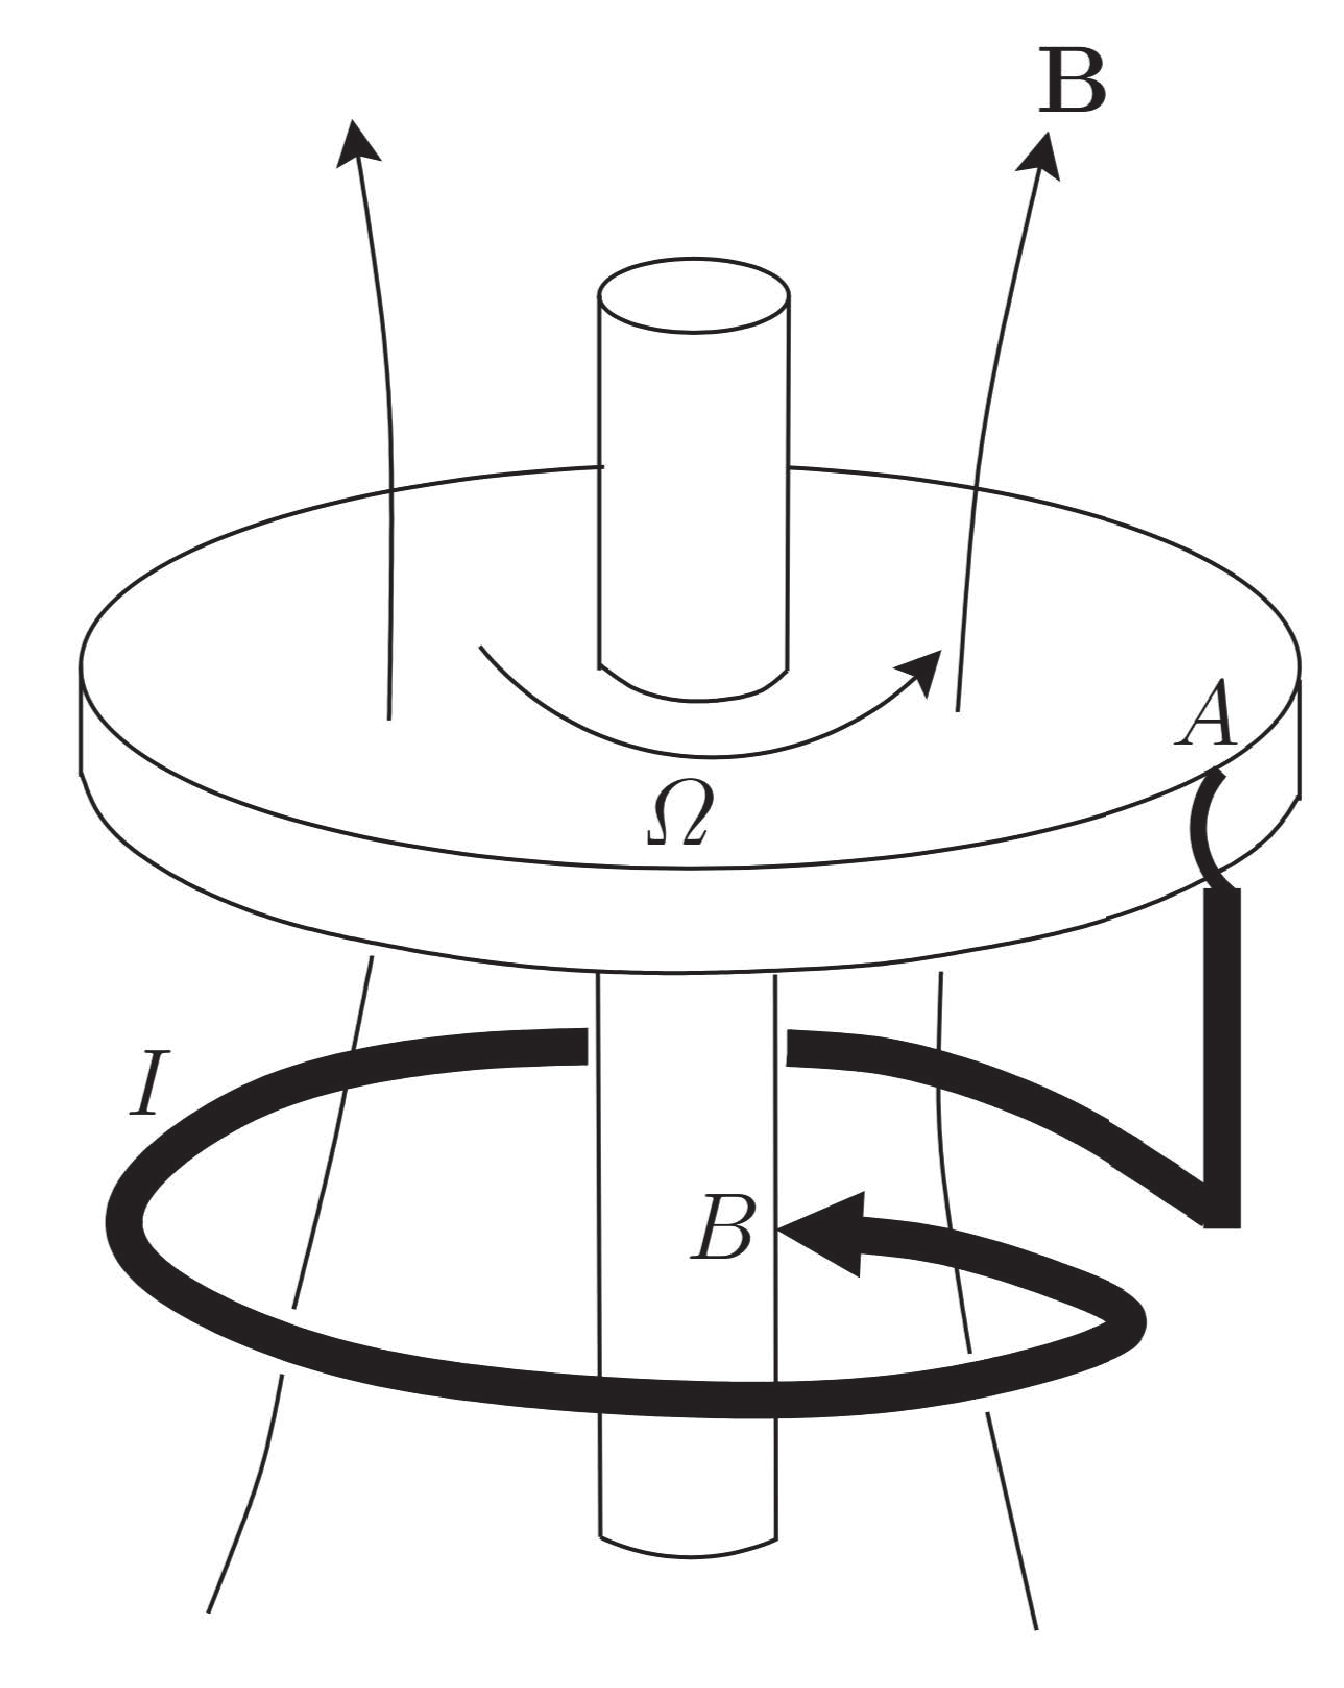
\includegraphics[height=10.cm, angle=0]{homopolar_disk_dynamo.eps}
\caption{
The homopolar disk dynamo.
}
\label{fig:homopolar}
\end{figure*}
%===========================================================================================================================


\section{Slow and Fast Dynamos}
\cite{Plasma2014} 







%%%%%%%%%%%%%%%%%%%%%%%%%%%%%%%%%%%%%%%%%%%%%%%%%%%%%%%%%%%%%%%%%%%%%%
\bibliographystyle{unsrt_update}
\bibliography{ref}
%%%%%%%%%%%%%%%%%%%%%%%%%%%%%%%%%%%%%%%%%%%%%%%%%%%%%%%%%%%%%%%%%%%%%%

\end{document}